\begin{minipage}{0.75\linewidth}
\begin{figure}[h]
    \centering
    \begin{adjustbox}{max width=1.0\linewidth, keepaspectratio}
        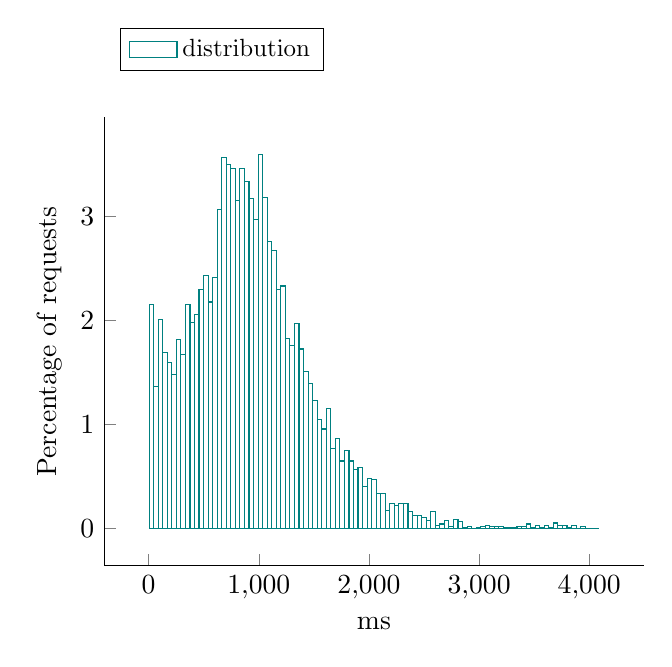
\begin{tikzpicture}
            \begin{axis}[ylabel = Percentage of requests, 
xlabel = ms, 
legend style = {nodes={scale=0.9, transform shape}, at={(0.03,1.2)}, anchor=north west, draw=black, fill=white, align=left, legend columns=3},
area style, mark size = 0pt,
 cycle list name = exotic,
  axis lines* = left]
		\addplot +[ybar interval] coordinates {
			 (4, 2.15716)
			 (45.24, 1.3662)
			 (86.48, 2.01335)
			 (127.72, 1.69492)
			 (168.96, 1.59219)
			 (210.2, 1.4792)
			 (251.44, 1.81818)
			 (292.68, 1.67437)
			 (333.92, 2.15716)
			 (375.16, 1.98254)
			 (416.4, 2.05444)
			 (457.64, 2.30098)
			 (498.88, 2.43451)
			 (540.12, 2.17771)
			 (581.36, 2.41397)
			 (622.6, 3.07139)
			 (663.84, 3.56446)
			 (705.08, 3.50282)
			 (746.32, 3.46174)
			 (787.56, 3.15357)
			 (828.8, 3.46174)
			 (870.04, 3.33847)
			 (911.28, 3.17411)
			 (952.52, 2.96867)
			 (993.76, 3.59527)
			 (1035, 3.18439)
			 (1076.24, 2.76323)
			 (1117.48, 2.67078)
			 (1158.72, 2.30098)
			 (1199.96, 2.33179)
			 (1241.2, 1.82845)
			 (1282.44, 1.75655)
			 (1323.68, 1.97227)
			 (1364.92, 1.72573)
			 (1406.16, 1.51002)
			 (1447.4, 1.39702)
			 (1488.64, 1.23267)
			 (1529.88, 1.04777)
			 (1571.12, 0.955316)
			 (1612.36, 1.15049)
			 (1653.6, 0.770416)
			 (1694.84, 0.862866)
			 (1736.08, 0.647149)
			 (1777.32, 0.749872)
			 (1818.56, 0.647149)
			 (1859.8, 0.564972)
			 (1901.04, 0.585516)
			 (1942.28, 0.400616)
			 (1983.52, 0.482794)
			 (2024.76, 0.472522)
			 (2066, 0.338983)
			 (2107.24, 0.338983)
			 (2148.48, 0.174628)
			 (2189.72, 0.236261)
			 (2230.96, 0.215716)
			 (2272.2, 0.236261)
			 (2313.44, 0.236261)
			 (2354.68, 0.164355)
			 (2395.92, 0.123267)
			 (2437.16, 0.123267)
			 (2478.4, 0.102722)
			 (2519.64, 0.0719055)
			 (2560.88, 0.164355)
			 (2602.12, 0.0308166)
			 (2643.36, 0.0410889)
			 (2684.6, 0.0719055)
			 (2725.84, 0.0205444)
			 (2767.08, 0.0821777)
			 (2808.32, 0.0616333)
			 (2849.56, 0.0102722)
			 (2890.8, 0.0205444)
			 (2932.04, 0)
			 (2973.28, 0.0102722)
			 (3014.52, 0.0205444)
			 (3055.76, 0.0308166)
			 (3097, 0.0205444)
			 (3138.24, 0.0205444)
			 (3179.48, 0.0205444)
			 (3220.72, 0.0102722)
			 (3261.96, 0.0102722)
			 (3303.2, 0.0102722)
			 (3344.44, 0.0205444)
			 (3385.68, 0.0205444)
			 (3426.92, 0.0410889)
			 (3468.16, 0.0102722)
			 (3509.4, 0.0308166)
			 (3550.64, 0.0102722)
			 (3591.88, 0.0308166)
			 (3633.12, 0.0102722)
			 (3674.36, 0.0513611)
			 (3715.6, 0.0308166)
			 (3756.84, 0.0308166)
			 (3798.08, 0.0102722)
			 (3839.32, 0.0308166)
			 (3880.56, 0)
			 (3921.8, 0.0205444)
			 (3963.04, 0)
			 (4004.28, 0)
			 (4045.52, 0)
			 (4086.76, 0)
		};
\addlegendentry{distribution};
           \end{axis}
      \end{tikzpicture}
  \end{adjustbox}
  \caption{Response time distribution - req = ReadUser-1}
\end{figure}
\end{minipage}\hfill\begin{minipage}{0.18\linewidth}
\begin{table}[h]
\begin{tabular}{|cc|}
\hline
\textbf{} & \textbf{ms}\\ \hline
 \Xhline{0.005\arrayrulewidth}
min & 4\\
 \Xhline{0.005\arrayrulewidth}
max & 4128\\
 \Xhline{0.005\arrayrulewidth}
mean & 928\\
 \Xhline{0.005\arrayrulewidth}
std & 556\\
\hline
\hline
 \Xhline{0.005\arrayrulewidth}
25th & 546\\
 \Xhline{0.005\arrayrulewidth}
50th & 877\\
 \Xhline{0.005\arrayrulewidth}
75th & 1226\\
 \Xhline{0.005\arrayrulewidth}
80th & 1333\\
 \Xhline{0.005\arrayrulewidth}
85th & 1458\\
 \Xhline{0.005\arrayrulewidth}
90th & 1634\\
 \Xhline{0.005\arrayrulewidth}
95th & 1925\\
 \Xhline{0.005\arrayrulewidth}
99th & 2562\\
\hline
\end{tabular}
\caption{Response time}
\end{table}
\end{minipage}\hfill